\documentclass{vldb}
\usepackage{graphicx}
\usepackage{balance}  % for  \balance command ON LAST PAGE  (only there!)
\usepackage[capposition=top]{floatrow}
\usepackage{float}
\usepackage[caption = false]{subfig}
%\usepackage{hyperref}

\begin{document}

% ****************** TITLE ****************************************

\title{On the Use of K-Competitive Networks \\ for Writing Style Transfer}

% ****************** AUTHORS **************************************

\numberofauthors{3} 

\author{
\alignauthor
Cameron Ibrahim\\
       \affaddr{Cornell University}\\
       \email{cai29@cornell.edu}
\alignauthor
Yuji Akimoto\\
       \affaddr{Cornell University}\\
       \email{ya242@cornell.edu}
\and
\alignauthor 
Ryan Butler\\
       \affaddr{Cornell University}\\
       \email{rjb392@cornell.edu}
\alignauthor 
Luca Leeser\\
       \affaddr{Cornell University}\\
       \email{ll698@cornell.edu}
}

\date{1 December 2017}

\maketitle

\begin{abstract}
Writing style is a key component of the quality of any online review - a detailed and informative review is only useful insofar as it is able to retain a reader's attention. In this paper, we explore the use of $k$-competitive layers in convolutional neural networks to classify the author of a given piece of text. We then apply the techniques used in neural style transfer for images to transfer the writing style of one author onto the content written by another. Given sufficient examples of well-written reviews, our techniques can be used to improve the quality of reviews on online platforms such as Yelp or Amazon.
\end{abstract}

% INTRODUCTION
\section{Introduction}
Neural style transfer \cite{GatysEB15a} has proven very successful at transferring the artistic style of an image onto the content of another. Due to the layered structure of convolutional neural networks, it was observed that later layers in the network produce feature representations of the content of an image, while the correlations between these features give a good representation of artistic style. More specifically, given a content image and style image, the algorithm treats the input to the network as a variable and simultaneously minimizes the $\ell_2$ norm between the input and content image's feature representations, and the input and style image's style representations.

\begin{figure}[h]
\subfloat{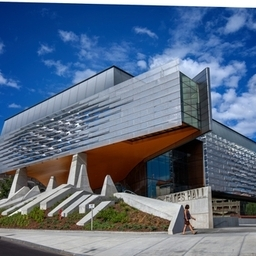
\includegraphics[width=.3\linewidth]{gates-hall.jpg}}
\hspace{0.1cm}
\subfloat{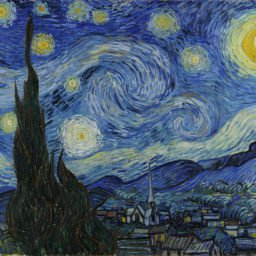
\includegraphics[width=.3\linewidth]{starry_night.jpg}}
\hspace{0.1cm}
\subfloat{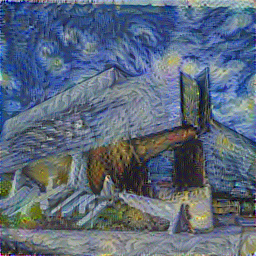
\includegraphics[width=.3\linewidth]{gates-starry.png}}
\caption{\textmd{Cornell's Gates Hall stylized in the form of Vincent Van Gogh's \textit{Starry Night}.}}
\end{figure} 

Modifications that optimize computational time \cite{JohnsonAL16}, preserve the texture of the style image \cite{GatysEB15}, and preserve facial structures in the content image \cite{KaurZD17}, among others, have further advanced the art of neural style transfer for images. However, applying similar techniques to text has proven difficult for a number of reasons. Firstly, textual data lives in an extremely sparse space, and therefore it is difficult to iteratively produce better stylized text while avoiding phrases that make no sense. Secondly, style and content are much more closely linked in text than they are in images - the same writer may write two passages of text in a completely different tone, yet maintain the same underlying style in a manner that is very subtle.

In this paper, we explore the use of $k$-competitive convolutional layers, a generalization of $k$-competitive layers designed for autoencoders in \cite{KATE}, which in turn are based on $k$-sparse layers as defined in \cite{MakhzaniF13}. We hypothesize that this technique will allow us to mitigate the high-dimensional sparsity of textual data and reduce the problem of writing style transfer to the well-established field of image style transfer. We integrate $k$-competitive layers into preprocessing and training of a word-level convolutional neural network \cite{Kim14f}, and perform a qualitative analysis of the quality of content and style representations generated by these networks. A key benefit of our method is that it does not require a training set of translations between writing styles, which are very difficult to obtain.

% RELATED WORK
\section{Related Work}
Early methods at quantitatively determining the writing style of a piece of text focused on statistical analyses of the rates of passive and active sentences, the ratio of pronouns to nouns to adjectives, and the likelihood of adjacent words given their distribution in the English language. However, these methods rely on unreliable tokenizations and are difficult to adapt to style transfer. Xu et. al. \cite{Xu12} provided some of the first algorithmic style transfer methods between Shakespearean and modern English, but relied on a phrase table and did not take advantage of modern machine learning methods. 

Recent methods based on neural networks fall into two broad categories: those that treat the problem as a mono-linguistic machine translation problem, and those that attempt to generate style and content representations of text.  \cite{Carlson17} and \cite{Jang16} fall under this first category, and generate stylized text that perform well according to BLEU score \cite{Papineni02}. However, these translation-based methods require a large dataset of tupled phrases that are identical in content and differ only in style. Use of passages in the Bible in \cite{Carlson17} and SparkNotes' Shakespearean translations in \cite{Jang16} present interesting but impractical test cases, while generating rap lyric translations with Google Translate via French \cite{Jang16} leaves much to be desired in terms of accuracy. 

\cite{Edirisooriya} and \cite{Kabbara16} both consider a similar method to ours in terms of generating style and content representations of text, and \cite{Kabbara16} defines three evaluation criteria: soundness (preservation of content), coherence (grammatical correctness \& common sense), and effectiveness (matches intended style). However, these lack sufficient experiments with which to evaluate the quality of their results. \cite{Fu17} provides a quantitative assessment of their content and style representations, in addition to a more complex alternative architecture. All of the aforementioned works use a recurrent neural network encoder-decoder structure (otherwise referred to as a ``seq2seq'' model), with either a long short-term memory (LSTM) or gated recurrent unit (GRU) used as the underlying structure. These methods seek to encode the content of the input text into a low dimensional space, and then use the decoder to generate text in a specified style. Our key contribution is in the use of convolutional neural networks, which have proven very successful at tasks such as sentiment analysis \cite{Kim14f}.

% PRELIMINARY ANALYSIS
\section{Preliminary Analysis}
The majority of implementations of style transfer for images use the VGG-19 \cite{VGG19} architecture to generate content and style representations of an image. This network was trained to classify images into one of the one thousand classes of the ImageNet challenge dataset \cite{ILSVRC15} and therefore is able to generate informative feature representations of a very large variety of objects. Given the resources required to train a similarly robust classifier for text, we first explore the tradeoffs of using an underlying network that is trained to discriminate between a much smaller number of classes by training a VGG network with the CIFAR-10 dataset \cite{Krizhevsky09} (here, we use pre-trained weights provided by \cite{Liu15}). Although this modified network is far less generalizable in terms of classification, we found that the content representations provided by later layers of the network were still informative enough to reconstruct the original image, even for images containing objects not included in the ten classes of CIFAR-10. By reconstruction, we refer to treating the input to the network as a variable, and minimizing $\ell_2$ loss between the input image and original image's feature representations in a certain layer.

\begin{figure}[h]
\subfloat{
\includegraphics[width=.15\linewidth]{cornell-campus-small.jpg}}
\hspace{0.1cm}
\subfloat{
\includegraphics[width=.15\linewidth]{anderson-small.jpg}}
\hspace{0.1cm}
\subfloat{
\includegraphics[width=.15\linewidth]{boats.jpg}}
\hspace{0.1cm}
\subfloat{
\includegraphics[width=.15\linewidth]{whale.jpg}}
\hspace{0.1cm} 
\subfloat{
\includegraphics[width=.15\linewidth]{pizza.jpg}}
\hspace{0.1cm} \\
\subfloat{
\includegraphics[width=.15\linewidth]{2600.png}}
\hspace{0.1cm}
\subfloat{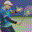
\includegraphics[width=.15\linewidth]{anderson5800.png}}
\hspace{0.1cm}
\subfloat{
\includegraphics[width=.15\linewidth]{boats2100.png}}
\hspace{0.1cm}
\subfloat{
\includegraphics[width=.15\linewidth]{boats3200.png}}
\hspace{0.1cm}
\subfloat{
\includegraphics[width=.15\linewidth]{pizza5000.png}}
\hspace{0.1cm} \\
\subfloat{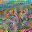
\includegraphics[width=.15\linewidth]{corne9900.png}}
\hspace{0.1cm}
\subfloat{
\includegraphics[width=.15\linewidth]{ander9900.png}}
\hspace{0.1cm}
\subfloat{
\includegraphics[width=.15\linewidth]{boats9900.png}}
\hspace	{0.1cm}
\subfloat{
\includegraphics[width=.15\linewidth]{whale9900.png}}
\hspace{0.1cm}
\subfloat{
\includegraphics[width=.15\linewidth]{pizza9900.png}}
\hspace{0.1cm}
\caption{\textmd{Several 32x32 images (top) reconstructed in the conv2\_2 layer (middle) and conv4\_2 layer (bottom) of VGG-19 trained on CIFAR-10 data; maximum 10000 iterations.}}
\end{figure} 

In the reconstruction phase, we use average-pooling in place of max-pooling, as suggested in \cite{GatysEB15a}. Although none of the images in Figure 2 resemble any of the ten classes present in CIFAR-10 data, the network still produces highly informative feature representations through convolution. This is a key observation in making the transition to text data, as writing style is subjective and therefore it is difficult to collect data from a large number of distinct classes that span the entire space of writing styles. 

However, we also observe that this reduction in generalizability of the underlying network architecture is not without tradeoffs. When using conv4\_2 as the layer at which to match the feature representations of two images (the layer used in Figure 1), the reconstructed images are mostly unrecognizable, and it takes a much larger number of iterations to produce something even remotely close to the original. However, we believe that there is enough signal even within the unrecognizable images, and with further hyperparameter optimization we will be able to mitigate this loss in reconstruction accuracy. This justifies the use of networks for author classification that have been trained on a limited number of classes as a starting point.

% MODEL
\section{Model}
\subsection{Convolutional Neural Networks for Text Classification}
Although recurrent neural networks have proven adept at language recognition tasks, evaluating the overall content and style of written text is a task that is less dependent on sequential information (outside the scope of a receptive field), and a hidden state is likely too small to encode enough information for our purposes. We believe that a a convolutional neural network allows us to take advantage of the success of style transfer for images, in contrast to aforementioned approaches that treat style transfer as a machine translation problem.

As the baseline for our comparisons we use a word-level convolutional neural network as designed by Yoon Kim in \cite{Kim14f}. A 1-d convolutional layer varies from those commonly found in architectures for image classification in that the receptive field of a filter is one-dimensional, and subsequent pooling layers operate along the time axis. The network takes as input a sentence, with each word encoded as a vector. As a ``shallow'' architecture, the network performs layer of convolution with filter lengths of 3, 4, 5 with 100 feature maps each, before a max-over-time pooling operation and a softmax layer. 

\begin{figure}[h]
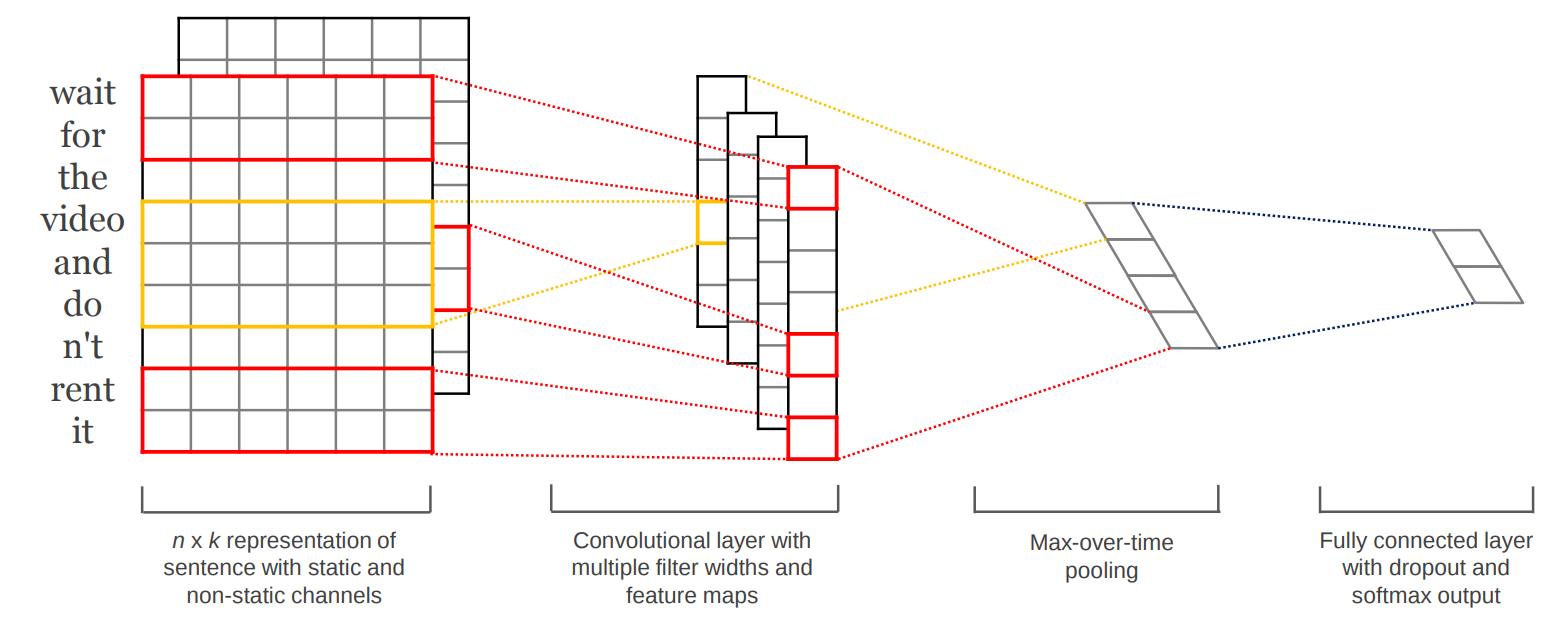
\includegraphics[width=\linewidth]{cnn.png}
\caption{\textmd{Structure of the baseline convolutional neural network model.}}
\end{figure}

\subsection{K-Competitive Convolutional Layers}
It has been observed that encouraging sparsity when learning representations acts as a capable reguarlizer that improves performance on classification tasks. In \cite{MakhzaniF13}, Makhzani and Frey designed the $k$-sparse autoencoder and demonstrated its effectiveness as a preprocessing step on image data. In the feedforward phase, sparsity is used as the sole non-linearity: after computing the activations $z = W^Tx + b$, only the largest $k$ entries of $z$ are kept and the rest are set to 0. 

Since textual data often has high-dimensionality, sparsity, and power-law distributions \cite{KATE}, autoencoders for text have often learned trivial features such as proper nouns specific to a certain passage. Chen and Zaki made a modification to $k$-sparse layers by introducing competition in the place of truncation: after computing the activations $z = tanh(W^Tx + b)$, only the $k$ entries with the largest absolute value are kept non-zero. These $k$ most ``competitive'' neurons are then augmented (with an amplification constant) with the \textbf{energy} of the ``losers'' that were made inactive, where the energy of a subset of neurons $H$ is defined as $\sum_{h_i \in H} |z_i|$. 

\begin{figure}[h]
\centering
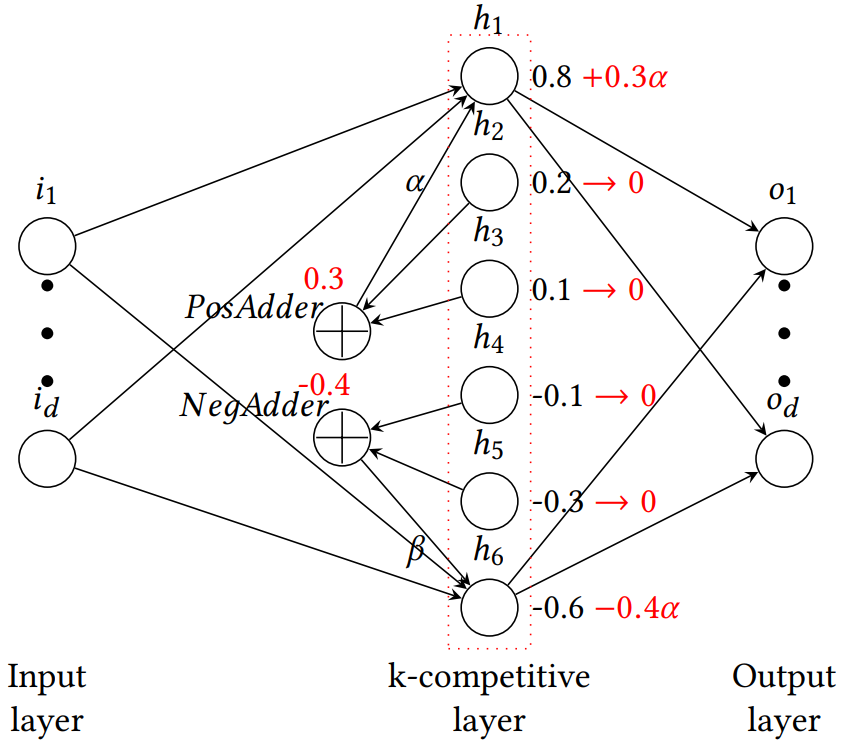
\includegraphics[width=.8\linewidth]{k_complayer.png}
\caption{\textmd{A fully connected $k$-competitive layer.}}
\end{figure}

Here, we propose a generalization of $k$-competitive layers to convolutional layers. Let $z_{ijk}$ be the activation volume produced by a convolutional layer, where $z_{x,y,:}$ denotes the feature vector at spatial location $(x,y)$. Then, we define the \textbf{energy map} of an activation volume, $E$, as the matrix with entries:
$$e_{ij} = \sum_{k=1}^K |z_{ijk}|$$
We then perform a $k$-competitive non-linearity, where we select the $k$ most competitive entries, and masking the activations of the ``loser'' neurons while augmenting the activations of the ``winner'' neurons. If we denote the set of indices of the $k$ ``winner'' neurons by $C_k$, then:
$$kcomp(z)_{i,j,:} = \textbf{0} \hspace{0.5cm} \forall (i,j) \notin C_k$$
$$kcomp(z)_{i,j,:} = z_{i,j,:} + \alpha\sum_{(i,j) \notin C_k} z_{i,j,:} \hspace{0.5cm} \forall (i,j) \in C_k$$
where $\alpha$, the amplification constant, is a hyperparameter.

% EXPERIMENTS
\section{Experiments}
\subsection{Datasets}
We use the most prolific reviewers on Yelp\footnote{{\texttt{https://www.yelp.com/dataset/challenge}}} to generate a large amounts of text for various styles of writing. Although the reviews for a frequent user of Yelp may span a number of years, we make the assumption that a user's writing style remains constant over that period of time. This may not strictly be the case as language, particularly of the colloquial variety that is often found online, evolves over time and certain words serve as clear indicators of certain time periods. However, dealing with a time-varying vocabulary set is an extension that we have not yet considered. After identifying the most frequent reviewers, we tokenize all of their reviews using NLTK \cite{Loper02nltk:the} to generate a corpus. To create a baseline task, we also create a corpus of Shakespearean works from Project Gutenberg\footnote{{\texttt{https://www.gutenberg.org/}}}. 

\subsection{Comparison of Architectures}
We explore the use of $k$-competitive layers in two settings: in an autoencoder to generate word embeddings, and as a non-linearity after convolutional layers. 

\subsubsection{K-Competitive Autoencoder for Embeddings}
In natural language processing tasks it is common encode textual data into a sparse space before generating embeddings that project these word or sentence-level vectors into a lower dimensional space. The $k$-competitive autoencoder for text (KATE) proposed in \cite{KATE} generates word embeddings that compare favorably to the more commonly used word2vec \cite{Mikolov13}, and we explore its use as a preprocessing step for an convolutional author classifier network. The two variants that we explore are in the initial sparse representation of training data: we compare between the use of a sentence-level log-normalized word count vectors similar to \cite{KATE} and word-level one-hot encoded vectors. 

Since the autoencoder is used to generate vector embeddings of words, it can be argued that using sentence-level embeddings as training data creates a model that is asked to perform different tasks at training and test time. At the same time, these log-normalized word count vectors contain entries between 0 and 1, and can therefore be interpreted as probabilities of potentially overlapping classes. Compared to the one-hot encoding approach that treats words as belonging in mutually exclusive classes, this approach more accurately reflects the reality that words often have overlapping meanings. The amount of training data produced from a single passage of text depends on the relative magnitudes of the number of unique words and number of unique sentences, but given an even ratio the word count approach likely produces more useful data - a single word is much more likely to be meaningless noise than a sentence.

Consistent with the probabilistic interpretation mentioned above, we swap the sigmoid activation function used in the word count approach for a softmax function when using one-hot encoding. We explore the tradeoffs between these two approaches, and quantitatively assess their performance by comparing reconstruction accuracy of the autoencoder, that is, the $\ell_2$ loss between the input vector and the decoded vector of its low dimensional representation.

\subsubsection{K-Competitive Layer as Activation Function}
Both convolutional and fully connected $k$-competitive layers are non-linear functions and are therefore appropriate as activation functions. Since they set the activations of the least active neurons to 0, these act similarly to a rectified linear unit with an adaptive threshold. As with ReLU, this property enforces sparsity among the coefficients and therefore acts both as a regularizer and non-linearity. Meanwhile, the allocation of energy from ``loser'' to ``winner'' nodes prevents these neurons from becoming entirely dead and preserves gradient flow in backpropagation. Since the baseline convolutional architecture is shallow and only has one convolutional layer (albeit many filters), we add one $k$-competitive layer following the convolutional layer, with a ReLU layer following it to preserve the non-linearity at inference time (the $k$-competitive layer is defined as the identity function at test time in \cite{KATE}). The classification tasks are: the baseline tasks of differentiating Shakespearean text from the most prolific Yelp reviewer; differentiating between the two most prolific Yelp reviewers.

We compare the performance of the following model configurations on two author classification tasks: the baseline convolutional network with one-hot encoded vectors as input; the baseline convolutional neural network with KATE embedded vectors as input; a convolutional neural network with a $k$-competitive layer taking one-hot encoded vectors as input.

\subsection{Hyperparameters and Training}
All models were implemented in TensorFlow and trained on a TITAN Xp GPU. Our implementation of the convolutional neural network from \cite{Kim14f} is credited to Denny Britz\footnote{{\texttt{https://github.com/dennybritz}}}. Both variations of the $k$-competitive autoencoder were trained with a bottleneck layer of size 128, $k=32$, amplification constant $\alpha=6.26$ \cite{KATE}, learning rate 0.001, 100 epochs, and a batch size of 128 using the Adam optimizer \cite{KingmaB14}. All variations of the convolutional network were trained with dropout rate 0.5, $\ell_2$ regularization parameter $\lambda=0$, learning rate 0.001, 200 epochs, and a batch size of 64 using the Adam optimizer. Variations with the $k$-competitive layer used $k=32, 64$ and $\alpha=6.26$.

% RESULTS
\section{Results}

% CONCLUSION
\section{Conclusion}

% FURTHER DISCUSSION
\section{Future Extensions}
Varying length of what is considered a single ``document'' on which to generate word count vector for KATE.

% ACKNOWLEDGMENTS 
\section{Acknowledgments}
The authors would like to thank Professor Thorsten Joachims at the department of Computer Science at Cornell University for his guidance, and their fellow members of the Cornell Data Science NLP Research Team for their support.


\bibliographystyle{abbrv}
\bibliography{sources.bib} 

% APPENDIX
\begin{appendix}
All code associated with this paper can be found here.
\end{appendix}

\balance

\end{document}